%%%%%%%%%%%%%%%%%%%%%%%%%%%%%%%%%%%%%%%%%
% Tutorial
% LaTeX Template
% Version 1.0 (05/11/17)
%
% Author:
% Ben Roose (ben.roose@wichita.edu)
%
% Original template author:
% Adam Glesser (adamglesser@gmail.com)
% www.LaTeXTemplates.com
%
% License:
% CC BY-NC-SA 3.0 (http://creativecommons.org/licenses/by-nc-sa/3.0/)
%
%%%%%%%%%%%%%%%%%%%%%%%%%%%%%%%%%%%%%%%%%

\documentclass[12pt]{article}

\usepackage{graphicx} %Allow import of images
\graphicspath{ {images/} } % Relative path to images directory
\usepackage[margin=1in]{geometry} % Required to make the margins smaller to fit more content on each page
\usepackage[linkcolor=blue]{hyperref} % Required to create hyperlinks to questions from elsewhere in the document
\hypersetup{pdfborder={0 0 0}, colorlinks=true, urlcolor=blue} % Specify a color for hyperlinks
\usepackage{todonotes} % Required for the boxes that questions appear in
\usepackage{tocloft} % Required to give customize the table of contents to display questions
\usepackage{microtype} % Slightly tweak font spacing for aesthetics
\usepackage{palatino} % Use the Palatino font

\setlength\parindent{0pt} % Removes all indentation from paragraphs

% Create and define the list of questions
\newlistof{questions}{faq}{\large FAQ for accessing the cslab-db MariaDB/MySQL service for CS 665} % This creates a new table of contents-like environment that will output a file with extension .faq
\setlength\cftbeforefaqtitleskip{3em} % Adjusts the vertical space between the title and subtitle
\setlength\cftafterfaqtitleskip{1em} % Adjusts the vertical space between the subtitle and the first question
\setlength\cftparskip{.3em} % Adjusts the vertical space between questions in the list of questions

% Create the command used for questions
\newcommand{\question}[1] % This is what you will use to create a new question
{
\refstepcounter{questions} % Increases the questions counter, this can be referenced anywhere with \thequestions
\par\noindent % Creates a new unindented paragraph
\phantomsection % Needed for hyperref compatibility with the \addcontensline command
\addcontentsline{faq}{questions}{#1} % Adds the question to the list of questions
\todo[inline, color=green!40]{\textbf{#1}} % Uses the todonotes package to create a fancy box to put the question
\vspace{1em} % White space after the question before the start of the answer
}

% Uncomment the line below to get rid of the trailing dots in the table of contents
%\renewcommand{\cftdot}{}

% Uncomment the two lines below to get rid of the numbers in the table of contents
%\let\Contentsline\contentsline
%\renewcommand\contentsline[3]{\Contentsline{#1}{#2}{}}

\begin{document}

%----------------------------------------------------------------------------------------
%	TITLE AND LIST OF QUESTIONS
%----------------------------------------------------------------------------------------

\begin{center}
\Huge{\bf \emph{EECS Tutorial: cslab-db MariaDB/MySQL service}} % Main title
\end{center}

\listofquestions % This prints the subtitle and a list of all of your questions
\bigskip % Create a gap between list and first question

\newpage % Comment this if you would like your questions and answers to start immediately after table of questions

%----------------------------------------------------------------------------------------
%	QUESTIONS AND ANSWERS
%----------------------------------------------------------------------------------------
\begin{flushleft}

\question{How do I access the \textit{phpMyAdmin} interface for cslab-db from a web-browser?}\label{phpmyadmin_access}

\begin{enumerate}
  \item Open your favorite web-browser and go to the cslab-db-web \textit{phpMyAdmin} interface at \href{http://cslab-db-web.cs.wichita.edu/}{cslab-db-web.cs.wichita.edu}
  \item At the login screen enter the dbuser\# and password given to you by your course instructor and you will be presented with the \textit{phpMyAdmin} home screen.
  \item You will have access to create, modify, insert, and delete tables, fields, and queries within the \verb|dbuser#_database| assigned to you for your course project.
  \item You can also use a MySQL console at the bottom of the \textit{phpMyAdmin} home screen.
  \item To log out of the \textit{phpMyAdmin} interface, click on the \textit{log out} icon under the logo on upper left of the window.
  \item For further information on how to use \textit{phpMyAdmin}, see \href{https://www.siteground.com/tutorials/phpmyadmin/}{phpMyAdmin tutorials}.
\end{enumerate}

\textbf{NOTE:} Due to WSU security policies, cslab-db-web can only be remotely accessed from on campus in the labs or after connecting into the university VPN service at \href{https://vpn.wichita.edu}{vpn.wichita.edu}.

\begin{figure}[h]
\caption{Example \textit{phpMyAdmin} home screen when you first log into cslab-db-web}
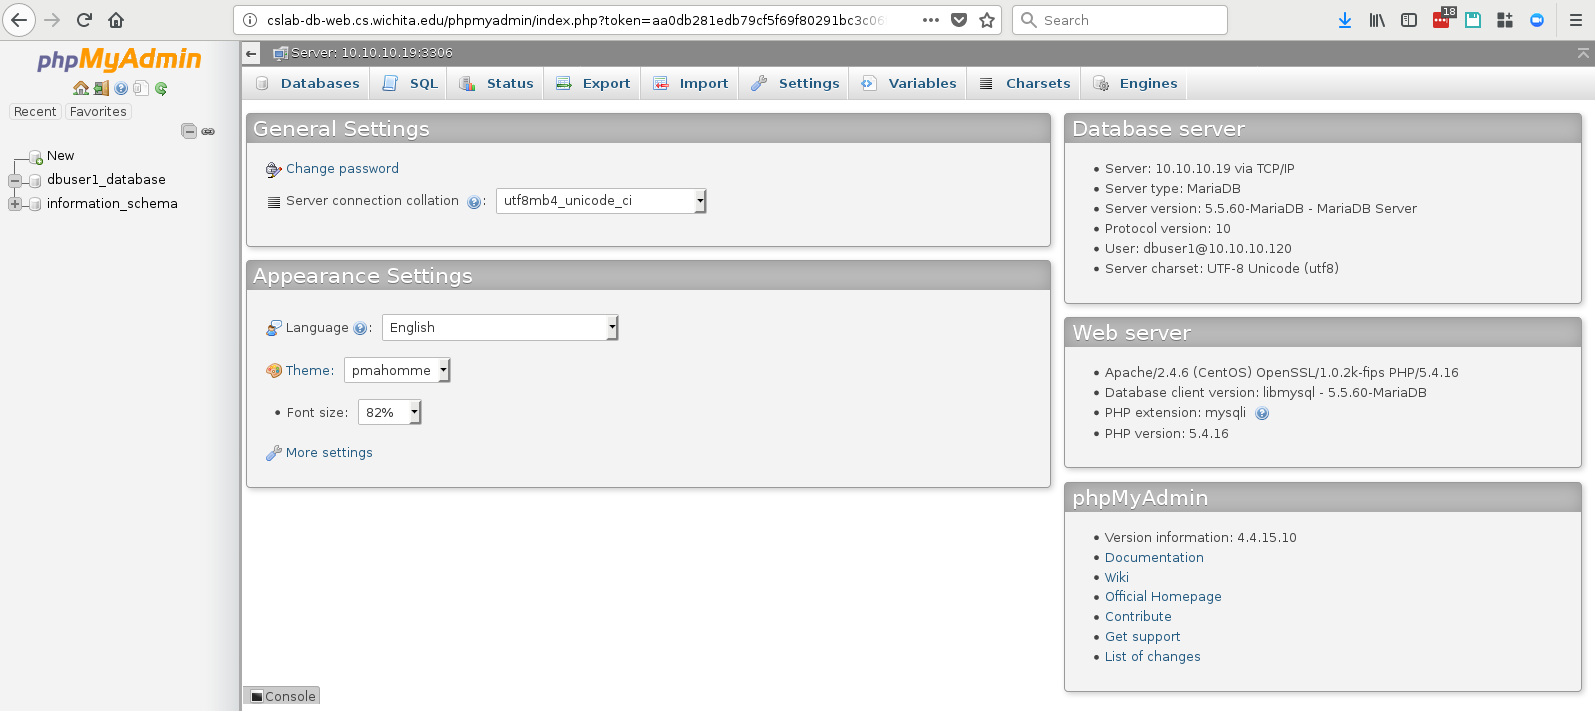
\includegraphics[width=\linewidth]{cslab-db_phpmyadmin_initial_homescreen}
\centering
\end{figure}

\newpage
%------------------------------------------------

\question{How do I access cslab-db using MySQL shell from the cslab Linux environment?}\label{mysql_shell_access}

\begin{enumerate}
  \item Follow the \href{https://github.com/benroose/tutorials/blob/master/cslab_tutorials/eecs_tutorial_cslab_web_access.pdf}{eecs\_tutorial\_cslab\_web\_access} document to log into \href{https://cslab-gateway.cs.wichita.edu/}{cslab-gateway.cs.wichita.edu} using a web-browser.
  \item Once logged into cslab \textit{guacamole}, open either a \textbf{cslab\_RDP\_GUI\_desktop} or \textbf{cslab\_SSH\_CLI\_terminal} connection.
  \item If you are using a \textbf{cslab\_RDP\_GUI\_desktop} connection, then open a terminal emulator window, such as \textit{LXTerminal} or \textit{Terminator}. 
  \item Alternatively, you can directly SSH into a cslab node if you have previously configured your SSH client. For further information on configuring an SSH client to access cslab, please follow the \href{https://github.com/benroose/tutorials/blob/master/cslab_tutorials/eecs_tutorial_cslab_ssh_access.pdf}{eecs\_tutorial\_cslab\_ssh\_access} document.
  \item Connect directly to the cslab-db MariaDB server from the cslab terminal by typing (where \texttt{\#} is the dbuser assigned to you by your course instructor) \break
    \verb|mysql -h cslab-db.cs.wichita.edu -D dbuser#_database -u dbuser# -p|
  \item Enter the password given to you by your instructor when prompted to do so.
  \item Once connected to cslab-db, you can use MariaDB/MySQL shell commands to create, modify, insert, and delete tables, fields, and queries within the \verb|dbuser#_database| assigned to you for your course project.
  \item To exit from the mysql shell, type \verb|exit| or press CTRL+D.
  \item For further information on how to use MariaDB/MySQL commands, please see the \href{https://mariadb.com/kb/en/library/training-tutorials/}{MariaDB Training \& Tutorials knowledge base}.
  \item For further information on the mysql shell command and associated option flags, please see the \href{https://linux.die.net/man/1/mysql}{official mysql man page}.
\end{enumerate}

%------------------------------------------------
\question{What do I do if I cannot access the cslab Linux environment? }\label{cslab_problems}
\begin{itemize}
  \item If you cannot access the cslab environment, ensure you have changed your myWSU password within the last three months and can access the myWSU main website \href{https://mywsu.wichita.edu}{mywsu.wichita.edu}. If you cannot access the myWSU website, then you will need to change your password before gaining access into the cslab environment.
  \item If you can access myWSU but cannot access the cslab environment, please contact the EECS systems administrator, \href{mailto:ben.roose@wichita.edu}{ben.roose@wichita.edu}.
\end{itemize}

%------------------------------------------------

\question{How do I embed SQL queries in my code/program for running within the cslab Linux environment?}\label{mysql_connector}

\begin{enumerate}
  \item Follow the \href{https://github.com/benroose/tutorials/blob/master/cslab_tutorials/eecs_tutorial_cslab_web_access.pdf}{eecs\_tutorial\_cslab\_web\_access} document to log into \href{https://cslab-gateway.cs.wichita.edu/}{cslab-gateway.cs.wichita.edu} using a web-browser.
  \item Once logged into cslab \textit{guacamole}, open either a \textbf{cslab\_RDP\_GUI\_desktop} or \textbf{cslab\_SSH\_CLI\_terminal} connection.
  \item Alternatively, you can directly SSH into a cslab node if you have previously configured your SSH client. For further information on configuring an SSH client to access cslab, please follow the \href{https://github.com/benroose/tutorials/blob/master/cslab_tutorials/eecs_tutorial_cslab_ssh_access.pdf}{eecs\_tutorial\_cslab\_ssh\_access} document.
  \item Code your C, C++, or Java program within cslab using a MariaDB/MySQL API connector. \break
  \item You will need to use the following details in your code to access your MySQL database (where \texttt{\#} is the dbuser assigned to you by your course instructor).
    \begin{itemize}
      \item \verb|host: cslab-db.cs.wichita.edu|
      \item \verb|port: 3306|
      \item \verb|database: dbuser#_database|
      \item \verb|user: dbuser#|
      \item \verb|password:| (the password assigned to you by your course instructor)
    \end{itemize}
  \item You will find a simple Java example using the MariaDB Connector/J with the standard Jave JDBC API in \href{https://github.com/benroose/cslab_db_java_test}{Ben Roose's GitHub repository here}.
  \item To compile and run Ben's Java example code, you will need to first clone/download his \verb|cslab_db_java_test| repository by typing \break
    \verb|git clone https://github.com/benroose/cslab_db_java_test.git|
  \item For further instructions on how to compile and run Ben's example code, follow the README.md file included within the newly cloned/downloaded directory.
  \item For further information on how to use MariaDB/MySQL API connectors, please see the \href{https://mariadb.com/kb/en/library/connectors/}{MariaDB Application Programming Interfaces documentation}.
  \item For questions on how to implement SQL queries within your code or if you wish to use a MySQL connector not currently installed within cslab, please speak with your course instructor.
\end{enumerate}

%------------------------------------------------ 

\end{flushleft}
\end{document}
